%%=============================================================================
%% LaTeX sjabloon voor bachelorproef, HoGent Bedrijf en Organisatie
%% Opleiding Toegepaste Informatica
%%=============================================================================

\documentclass[fleqn,a4paper,12pt]{book}

%%=============================================================================
%% LaTeX sjabloon voor de bachelorproef, HoGent Bedrijf en Organisatie
%% Opleiding toegepaste informatica
%%
%% Structuur en algemene vormgeving. Meestal hoef je hier niets te wijzigen.
%%
%% Vormgeving gebaseerd op "The Legrand Orange Book", version 2.0 (9/2/15)
%% door Mathias Legrand (legrand.mathias@gmail.com) met aanpassingen door
%% Vel (vel@latextemplates.com). Het oorspronkelijke template is te vinden op
%% http://www.LaTeXTemplates.com
%%
%% Aanpassingen voor HoGent toegepaste informatica: 
%%   Bert Van Vreckem <bert.vanvreckem@hogent.be>
%% Licentie: 
%%   CC BY-NC-SA 3.0 (http://creativecommons.org/licenses/by-nc-sa/3.0/)
%%=============================================================================

%%-----------------------------------------------------------------------------
%% Packages
%%-----------------------------------------------------------------------------

\usepackage[top=3cm,bottom=3cm,left=3cm,right=3cm,headsep=10pt,a4paper]{geometry} % Page margins
\usepackage[utf8]{inputenc}  % Accenten gebruiken in tekst (vb. é ipv \'e)
\usepackage{amsfonts}        % AMS math packages: extra wiskundige
\usepackage{amsmath}         %   symbolen (o.a. getallen-
\usepackage{amssymb}         %   verzamelingen N, R, Z, Q, etc.)
\usepackage[english,dutch]{babel}    % Taalinstellingen: woordsplitsingen,
                             %  commando's voor speciale karakters
                             %  ("dutch" voor NL)
\usepackage{iflang}
\usepackage{eurosym}         % Euro-symbool €
\usepackage{geometry}
\usepackage{graphicx}        % Invoegen van tekeningen
\graphicspath{{img/}}       % Specifies the directory where pictures are stored
\usepackage{tikz}            % Required for drawing custom shapes
\usepackage[pdftex,bookmarks=true]{hyperref}
                             % PDF krijgt klikbare links & verwijzingen,
                             %  inhoudstafel
\usepackage{enumitem}        % Customize lists
\setlist{nolistsep}         % Reduce spacing between list items
\usepackage{listings}        % Broncode mooi opmaken
\usepackage{multirow}        % Tekst over verschillende cellen in tabellen
\usepackage{rotating}        % Tabellen en figuren roteren

\usepackage{booktabs}        % Required for nicer horizontal rules in tables

\usepackage{xcolor}          % Required for specifying colors by name
\definecolor{maincolor}{RGB}{0,147,208} % Define the main color used for 
                             % highlighting throughout the book
                             % 0, 147, 208 = officiële kleur HoGent FBO

% Paragraph style: no indent, add space between paragraphs
\setlength{\parindent}{0em}
\setlength{\parskip}{1em}

\usepackage{etoolbox}
\usepackage{titling} % Macros for title, author, etc
\usepackage{lipsum}          % Voor vultekst (lorem ipsum)

%----------------------------------------------------------------------------------------
%	FONTS
%----------------------------------------------------------------------------------------

\usepackage{avant} % Use the Avantgarde font for headings
%\usepackage{times} % Use the Times font for headings
\usepackage{mathptmx} % Use the Adobe Times Roman as the default text font together with math symbols from the Sym­bol, Chancery and Com­puter Modern fonts

\usepackage{microtype} % Slightly tweak font spacing for aesthetics
\usepackage[utf8]{inputenc} % Required for including letters with accents
\usepackage[T1]{fontenc} % Use 8-bit encoding that has 256 glyphs

%------------------------------------------------------------------------------
%	TITLE PAGE
%------------------------------------------------------------------------------

\newcommand{\inserttitlepage}{%
\begin{titlepage}
  \newgeometry{top=2cm,bottom=1.5cm,left=1.5cm,right=1.5cm}
  \begin{center}

    \begingroup
    \rmfamily
    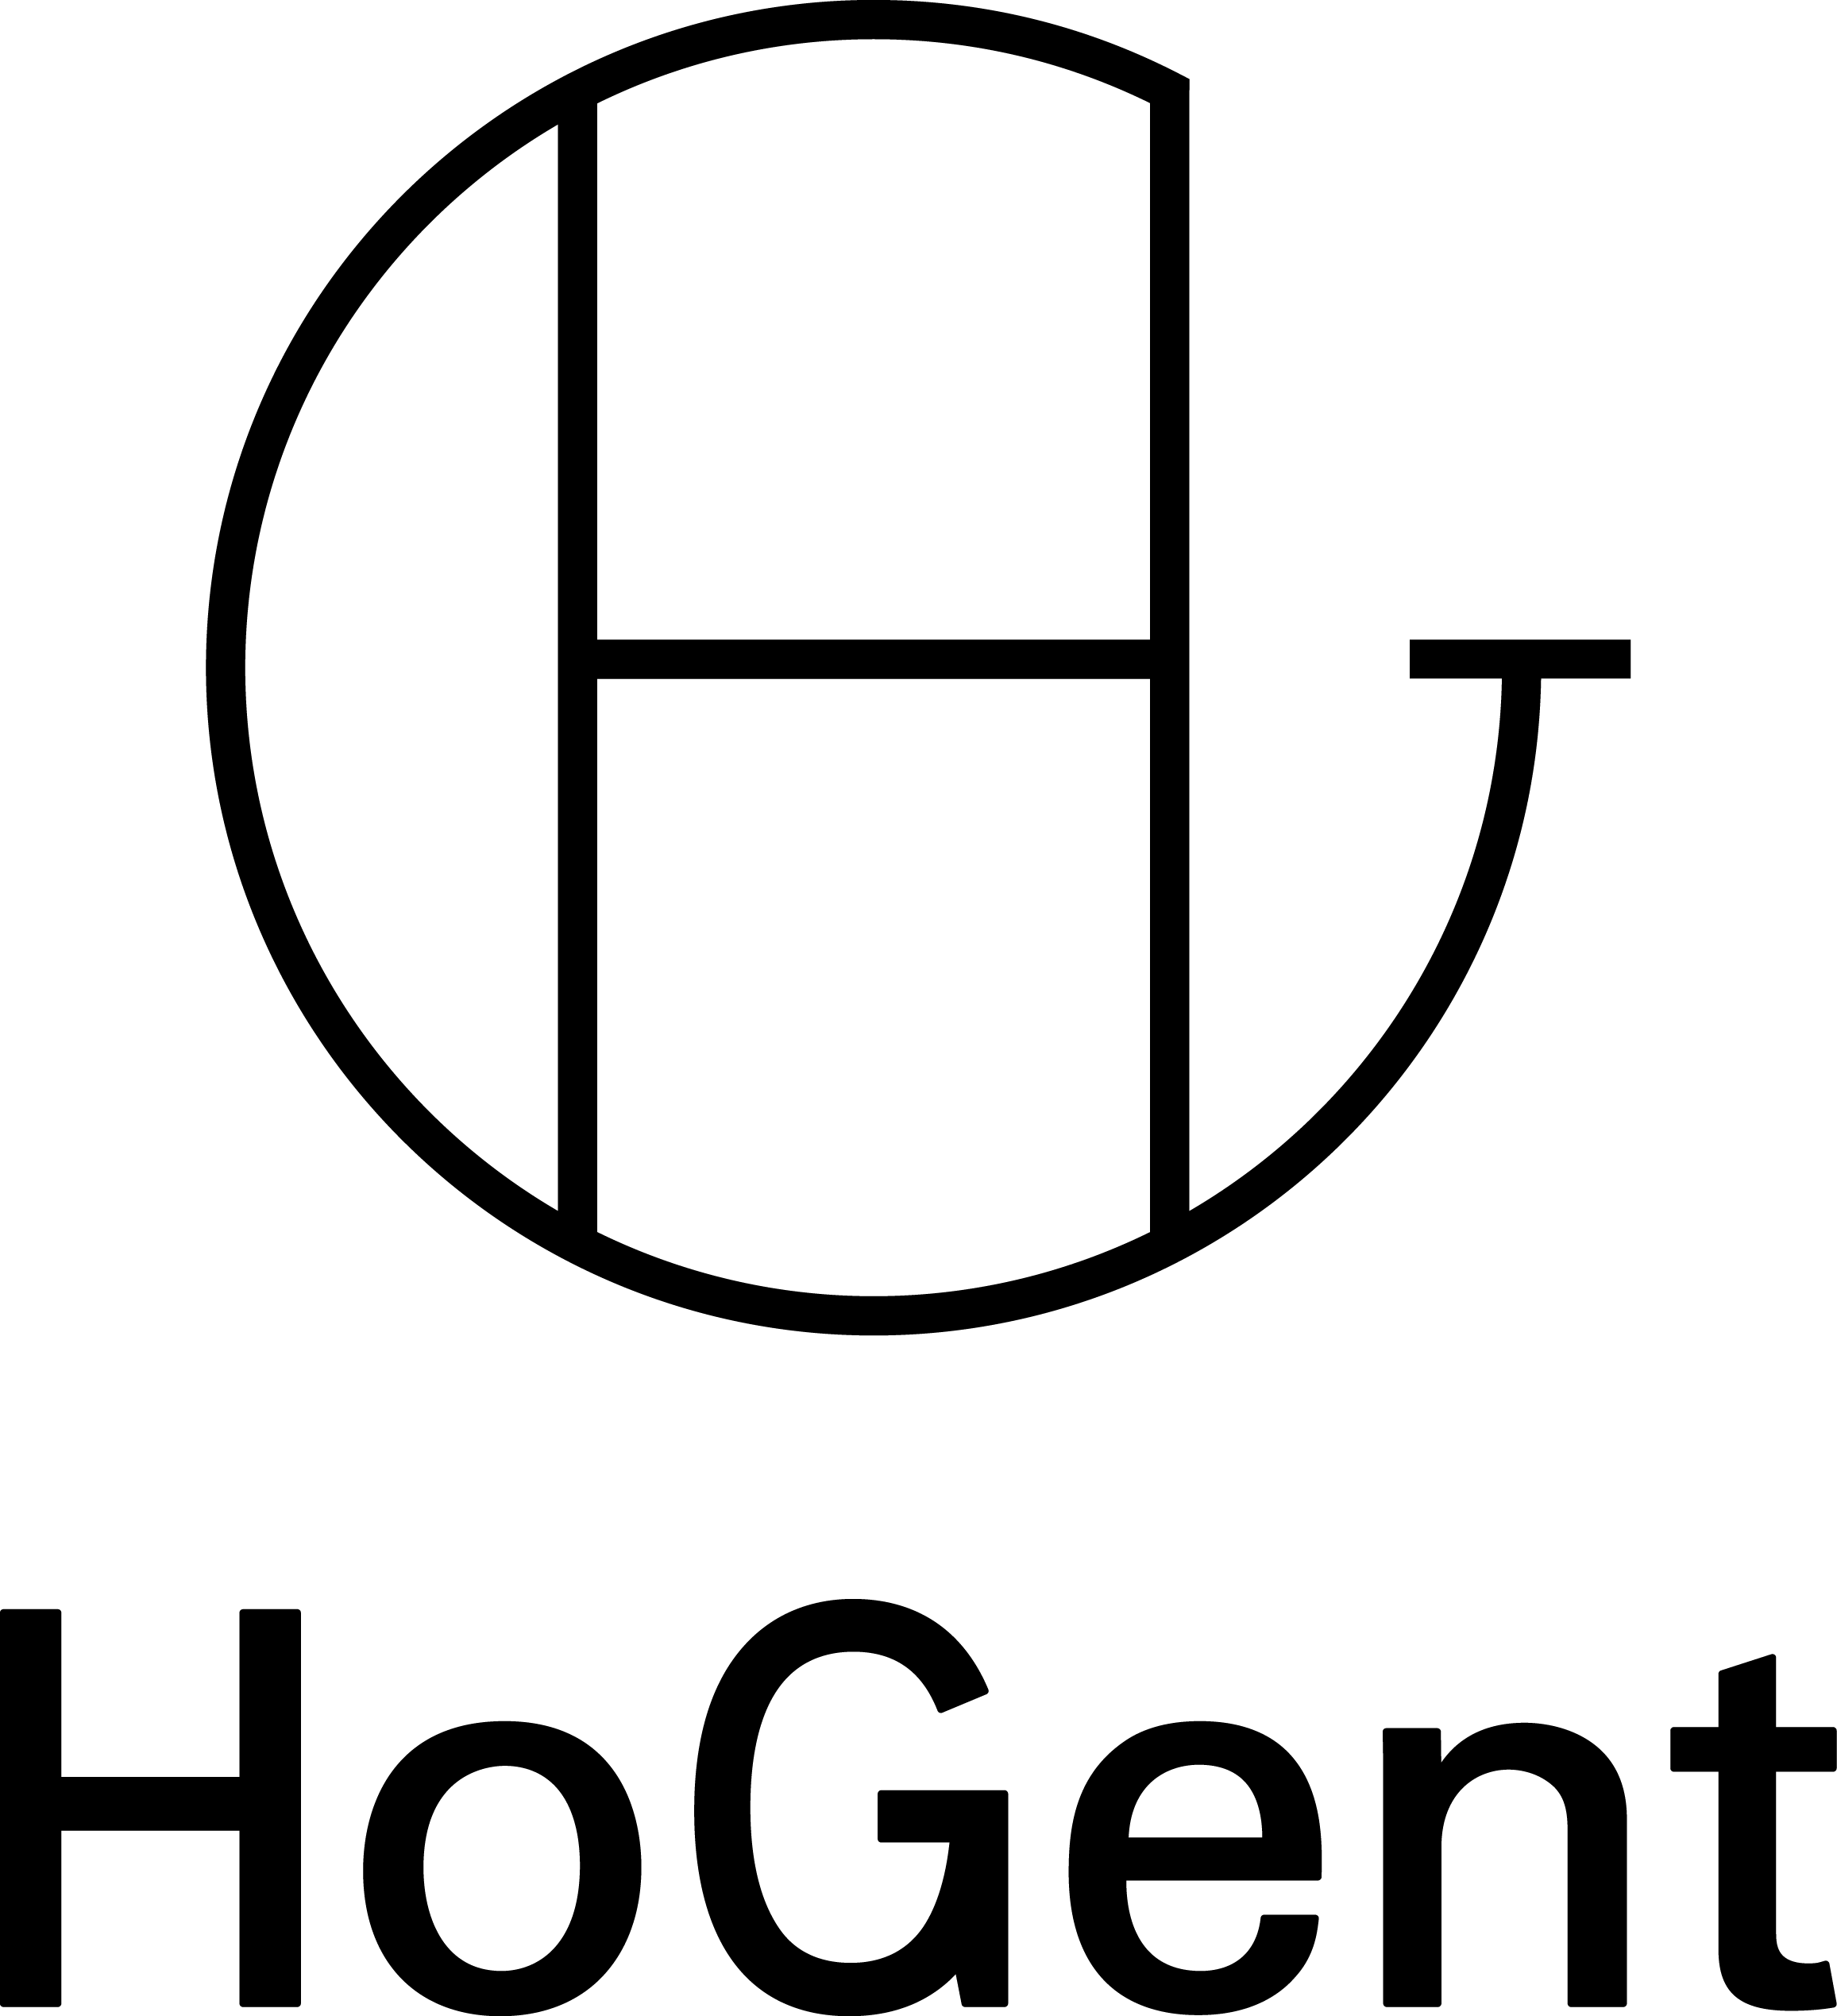
\includegraphics[width=2.5cm]{img/HG-beeldmerk-woordmerk}\\[.5cm]
    Faculteit Bedrijf en Organisatie\\[3cm]
    \titel
    \vfill
    \student\\[3.5cm]
    Scriptie voorgedragen tot het bekomen van de graad van\\professionele bachelor in de toegepaste informatica\\[2cm]
    Promotor:\\
    \promotor\\
    \ifdefempty{\copromotor}{\vspace{2.5cm}}{Co-promotor:\\\copromotor\\[2.5cm]}
    Instelling: \instelling\\[.5cm]
    Academiejaar: \academiejaar\\[.5cm]
    \ifcase \examenperiode \or Eerste \or Tweede \else Derde \fi examenperiode
    \endgroup

  \end{center}
  \restoregeometry
\end{titlepage}
  \emptypage
\begin{titlepage}
  \newgeometry{top=5.35cm,bottom=1.5cm,left=1.5cm,right=1.5cm}
  \begin{center}

    \begingroup
    \rmfamily
    \IfLanguageName{dutch}{Faculteit Bedrijf en Organisatie}{Faculty of Business and Information Management}\\[3cm]
    \titel
    \vfill
    \student\\[3.5cm]
    \IfLanguageName{dutch}{Scriptie voorgedragen tot het bekomen van de graad van\\professionele bachelor in de toegepaste informatica}{Thesis submitted in partial fulfillment of the requirements for the degree of\\professional bachelor of applied computer science}\\[2cm]
    Promotor:\\
    \promotor\\
    \ifdefempty{\copromotor}{\vspace{2.5cm}}{Co-promotor:\\\copromotor\\[2.5cm]}
    \IfLanguageName{dutch}{Instelling}{Institution}: \instelling\\[.5cm]
    \IfLanguageName{dutch}{Academiejaar}{Academic year}: \academiejaar\\[.5cm]
    \IfLanguageName{dutch}{%
    \ifcase \examenperiode \or Eerste \or Tweede \else Derde \fi examenperiode}{%
    \ifcase \examenperiode \or First \or Second \else Third \fi examination period}
    \endgroup

  \end{center}
  \restoregeometry
\end{titlepage}
}

%----------------------------------------------------------------------------------------
%	BIBLIOGRAPHY AND INDEX
%----------------------------------------------------------------------------------------

\usepackage[style=apa,backend=biber]{biblatex}
\usepackage{csquotes}
\DeclareLanguageMapping{dutch}{dutch-apa}
\addbibresource{bachproef-tin.bib} % BibTeX bibliography file
\defbibheading{bibempty}{}

\usepackage{calc} % For simpler calculation - used for spacing the index letter headings correctly
\usepackage{makeidx} % Required to make an index
\makeindex % Tells LaTeX to create the files required for indexing

%----------------------------------------------------------------------------------------
%	MAIN TABLE OF CONTENTS
%----------------------------------------------------------------------------------------

\usepackage{titletoc} % Required for manipulating the table of contents

\contentsmargin{0cm} % Removes the default margin

% Part text styling
\titlecontents{part}[0cm]
{\addvspace{20pt}\centering\large\bfseries}
{}
{}
{}

% Chapter text styling
\titlecontents{chapter}[1.25cm] % Indentation
{\addvspace{12pt}\large\sffamily\bfseries} % Spacing and font options for chapters
{\color{maincolor!60}\contentslabel[\Large\thecontentslabel]{1.25cm}\color{maincolor}} % Chapter number
{\color{maincolor}}
{\color{maincolor!60}\normalsize\;\titlerule*[.5pc]{.}\;\thecontentspage} % Page number

% Section text styling
\titlecontents{section}[1.25cm] % Indentation
{\addvspace{3pt}\sffamily\bfseries} % Spacing and font options for sections
{\contentslabel[\thecontentslabel]{1.25cm}} % Section number
{}
{\hfill\color{black}\thecontentspage} % Page number
[]

% Subsection text styling
\titlecontents{subsection}[1.25cm] % Indentation
{\addvspace{1pt}\sffamily\small} % Spacing and font options for subsections
{\contentslabel[\thecontentslabel]{1.25cm}} % Subsection number
{}
{\ \titlerule*[.5pc]{.}\;\thecontentspage} % Page number
[]

% List of figures
\titlecontents{figure}[0em]
{\addvspace{-5pt}\sffamily}
{\thecontentslabel\hspace*{1em}}
{}
{\ \titlerule*[.5pc]{.}\;\thecontentspage}
[]

% List of tables
\titlecontents{table}[0em]
{\addvspace{-5pt}\sffamily}
{\thecontentslabel\hspace*{1em}}
{}
{\ \titlerule*[.5pc]{.}\;\thecontentspage}
[]

%----------------------------------------------------------------------------------------
%	MINI TABLE OF CONTENTS IN PART HEADS
%----------------------------------------------------------------------------------------

% Chapter text styling
\titlecontents{lchapter}[0em] % Indenting
{\addvspace{15pt}\large\sffamily\bfseries} % Spacing and font options for chapters
{\color{maincolor}\contentslabel[\Large\thecontentslabel]{1.25cm}\color{maincolor}} % Chapter number
{}
{\color{maincolor}\normalsize\sffamily\bfseries\;\titlerule*[.5pc]{.}\;\thecontentspage} % Page number

% Section text styling
\titlecontents{lsection}[0em] % Indenting
{\sffamily\small} % Spacing and font options for sections
{\contentslabel[\thecontentslabel]{1.25cm}} % Section number
{}
{}

% Subsection text styling
\titlecontents{lsubsection}[.5em] % Indentation
{\normalfont\footnotesize\sffamily} % Font settings
{}
{}
{}

%----------------------------------------------------------------------------------------
%	PAGE HEADERS
%----------------------------------------------------------------------------------------

\usepackage{fancyhdr} % Required for header and footer configuration

\pagestyle{fancy}
\renewcommand{\chaptermark}[1]{\markboth{\sffamily\normalsize\bfseries\chaptername\ \thechapter.\ #1}{}} % Chapter text font settings
\renewcommand{\sectionmark}[1]{\markright{\sffamily\normalsize\thesection\hspace{5pt}#1}{}} % Section text font settings
\fancyhf{} \fancyhead[LE,RO]{\sffamily\normalsize\thepage} % Font setting for the page number in the header
\fancyhead[LO]{\rightmark} % Print the nearest section name on the left side of odd pages
\fancyhead[RE]{\leftmark} % Print the current chapter name on the right side of even pages
\renewcommand{\headrulewidth}{0.5pt} % Width of the rule under the header
\addtolength{\headheight}{2.5pt} % Increase the spacing around the header slightly
\renewcommand{\footrulewidth}{0pt} % Removes the rule in the footer
\fancypagestyle{plain}{\fancyhead{}\renewcommand{\headrulewidth}{0pt}} % Style for when a plain pagestyle is specified

% Removes the header from odd empty pages at the end of chapters
\makeatletter
\renewcommand{\cleardoublepage}{
\clearpage\ifodd\c@page\else
\hbox{}
\vspace*{\fill}
\thispagestyle{empty}
\newpage
\fi}

%----------------------------------------------------------------------------------------
%	THEOREM STYLES
%----------------------------------------------------------------------------------------

\usepackage{amsmath,amsfonts,amssymb,amsthm} % For math equations, theorems, symbols, etc

\newcommand{\intoo}[2]{\mathopen{]}#1\,;#2\mathclose{[}}
\newcommand{\ud}{\mathop{\mathrm{{}d}}\mathopen{}}
\newcommand{\intff}[2]{\mathopen{[}#1\,;#2\mathclose{]}}
\newtheorem{notation}{Notation}[chapter]

% Boxed/framed environments
\newtheoremstyle{maincolornumbox}% % Theorem style name
{0pt}% Space above
{0pt}% Space below
{\normalfont}% % Body font
{}% Indent amount
{\small\bf\sffamily\color{maincolor}}% % Theorem head font
{\;}% Punctuation after theorem head
{0.25em}% Space after theorem head
{\small\sffamily\color{maincolor}\thmname{#1}\nobreakspace\thmnumber{\@ifnotempty{#1}{}\@upn{#2}}% Theorem text (e.g. Theorem 2.1)
\thmnote{\nobreakspace\the\thm@notefont\sffamily\bfseries\color{black}---\nobreakspace#3.}} % Optional theorem note
\renewcommand{\qedsymbol}{$\blacksquare$}% Optional qed square

\newtheoremstyle{blacknumex}% Theorem style name
{5pt}% Space above
{5pt}% Space below
{\normalfont}% Body font
{} % Indent amount
{\small\bf\sffamily}% Theorem head font
{\;}% Punctuation after theorem head
{0.25em}% Space after theorem head
{\small\sffamily{\tiny\ensuremath{\blacksquare}}\nobreakspace\thmname{#1}\nobreakspace\thmnumber{\@ifnotempty{#1}{}\@upn{#2}}% Theorem text (e.g. Theorem 2.1)
\thmnote{\nobreakspace\the\thm@notefont\sffamily\bfseries---\nobreakspace#3.}}% Optional theorem note

\newtheoremstyle{blacknumbox} % Theorem style name
{0pt}% Space above
{0pt}% Space below
{\normalfont}% Body font
{}% Indent amount
{\small\bf\sffamily}% Theorem head font
{\;}% Punctuation after theorem head
{0.25em}% Space after theorem head
{\small\sffamily\thmname{#1}\nobreakspace\thmnumber{\@ifnotempty{#1}{}\@upn{#2}}% Theorem text (e.g. Theorem 2.1)
\thmnote{\nobreakspace\the\thm@notefont\sffamily\bfseries---\nobreakspace#3.}}% Optional theorem note

% Non-boxed/non-framed environments
\newtheoremstyle{maincolornum}% % Theorem style name
{5pt}% Space above
{5pt}% Space below
{\normalfont}% % Body font
{}% Indent amount
{\small\bf\sffamily\color{maincolor}}% % Theorem head font
{\;}% Punctuation after theorem head
{0.25em}% Space after theorem head
{\small\sffamily\color{maincolor}\thmname{#1}\nobreakspace\thmnumber{\@ifnotempty{#1}{}\@upn{#2}}% Theorem text (e.g. Theorem 2.1)
\thmnote{\nobreakspace\the\thm@notefont\sffamily\bfseries\color{black}---\nobreakspace#3.}} % Optional theorem note
\renewcommand{\qedsymbol}{$\blacksquare$}% Optional qed square
\makeatother

% Defines the theorem text style for each type of theorem to one of the three styles above
\newcounter{dummy}
\numberwithin{dummy}{section}
\theoremstyle{maincolornumbox}
\newtheorem{theoremeT}[dummy]{Theorem}
\newtheorem{problem}{Problem}[chapter]
\newtheorem{exerciseT}{Exercise}[chapter]
\theoremstyle{blacknumex}
\newtheorem{exampleT}{Example}[chapter]
\theoremstyle{blacknumbox}
\newtheorem{vocabulary}{Vocabulary}[chapter]
\newtheorem{definitionT}{Definition}[section]
\newtheorem{corollaryT}[dummy]{Corollary}
\theoremstyle{maincolornum}
\newtheorem{proposition}[dummy]{Proposition}

%----------------------------------------------------------------------------------------
%	DEFINITION OF COLORED BOXES
%----------------------------------------------------------------------------------------

\RequirePackage[framemethod=default]{mdframed} % Required for creating the theorem, definition, exercise and corollary boxes

% Theorem box
\newmdenv[skipabove=7pt,
skipbelow=7pt,
backgroundcolor=black!5,
linecolor=maincolor,
innerleftmargin=5pt,
innerrightmargin=5pt,
innertopmargin=5pt,
leftmargin=0cm,
rightmargin=0cm,
innerbottommargin=5pt]{tBox}

% Exercise box
\newmdenv[skipabove=7pt,
skipbelow=7pt,
rightline=false,
leftline=true,
topline=false,
bottomline=false,
backgroundcolor=maincolor!10,
linecolor=maincolor,
innerleftmargin=5pt,
innerrightmargin=5pt,
innertopmargin=5pt,
innerbottommargin=5pt,
leftmargin=0cm,
rightmargin=0cm,
linewidth=4pt]{eBox}

% Definition box
\newmdenv[skipabove=7pt,
skipbelow=7pt,
rightline=false,
leftline=true,
topline=false,
bottomline=false,
linecolor=maincolor,
innerleftmargin=5pt,
innerrightmargin=5pt,
innertopmargin=0pt,
leftmargin=0cm,
rightmargin=0cm,
linewidth=4pt,
innerbottommargin=0pt]{dBox}

% Corollary box
\newmdenv[skipabove=7pt,
skipbelow=7pt,
rightline=false,
leftline=true,
topline=false,
bottomline=false,
linecolor=gray,
backgroundcolor=black!5,
innerleftmargin=5pt,
innerrightmargin=5pt,
innertopmargin=5pt,
leftmargin=0cm,
rightmargin=0cm,
linewidth=4pt,
innerbottommargin=5pt]{cBox}

% Creates an environment for each type of theorem and assigns it a theorem text style from the "Theorem Styles" section above and a colored box from above
\newenvironment{theorem}{\begin{tBox}\begin{theoremeT}}{\end{theoremeT}\end{tBox}}
\newenvironment{exercise}{\begin{eBox}\begin{exerciseT}}{\hfill{\color{maincolor}\tiny\ensuremath{\blacksquare}}\end{exerciseT}\end{eBox}}
\newenvironment{definition}{\begin{dBox}\begin{definitionT}}{\end{definitionT}\end{dBox}}
\newenvironment{example}{\begin{exampleT}}{\hfill{\tiny\ensuremath{\blacksquare}}\end{exampleT}}
\newenvironment{corollary}{\begin{cBox}\begin{corollaryT}}{\end{corollaryT}\end{cBox}}

%----------------------------------------------------------------------------------------
%	REMARK ENVIRONMENT
%----------------------------------------------------------------------------------------

\newenvironment{remark}{\par\vspace{10pt}\small % Vertical white space above the remark and smaller font size
\begin{list}{}{
\leftmargin=35pt % Indentation on the left
\rightmargin=25pt}\item\ignorespaces % Indentation on the right
\makebox[-2.5pt]{\begin{tikzpicture}[overlay]
\node[draw=maincolor!60,line width=1pt,circle,fill=maincolor!25,font=\sffamily\bfseries,inner sep=2pt,outer sep=0pt] at (-15pt,0pt){\textcolor{maincolor}{R}};\end{tikzpicture}} % Orange R in a circle
\advance\baselineskip -1pt}{\end{list}\vskip5pt} % Tighter line spacing and white space after remark

%----------------------------------------------------------------------------------------
%	SECTION NUMBERING IN THE MARGIN
%----------------------------------------------------------------------------------------

\makeatletter
\renewcommand{\@seccntformat}[1]{\llap{\textcolor{maincolor}{\csname the#1\endcsname}\hspace{1em}}}
\renewcommand{\section}{\@startsection{section}{1}{\z@}
{-4ex \@plus -1ex \@minus -.4ex}
{1ex \@plus.2ex }
{\normalfont\large\sffamily\bfseries}}
\renewcommand{\subsection}{\@startsection {subsection}{2}{\z@}
{-3ex \@plus -0.1ex \@minus -.4ex}
{0.5ex \@plus.2ex }
{\normalfont\sffamily\bfseries}}
\renewcommand{\subsubsection}{\@startsection {subsubsection}{3}{\z@}
{-2ex \@plus -0.1ex \@minus -.2ex}
{.2ex \@plus.2ex }
{\normalfont\small\sffamily\bfseries}}
\renewcommand\paragraph{\@startsection{paragraph}{4}{\z@}
{-2ex \@plus-.2ex \@minus .2ex}
{.1ex}
{\normalfont\small\sffamily\bfseries}}

%----------------------------------------------------------------------------------------
%	PART HEADINGS
%----------------------------------------------------------------------------------------

% numbered part in the table of contents
\newcommand{\@mypartnumtocformat}[2]{%
\setlength\fboxsep{0pt}%
\noindent\colorbox{maincolor!20}{\strut\parbox[c][.7cm]{\ecart}{\color{maincolor!70}\Large\sffamily\bfseries\centering#1}}\hskip\esp\colorbox{maincolor!40}{\strut\parbox[c][.7cm]{\linewidth-\ecart-\esp}{\Large\sffamily\centering#2}}}%
%%%%%%%%%%%%%%%%%%%%%%%%%%%%%%%%%%
% unnumbered part in the table of contents
\newcommand{\@myparttocformat}[1]{%
\setlength\fboxsep{0pt}%
\noindent\colorbox{maincolor!40}{\strut\parbox[c][.7cm]{\linewidth}{\Large\sffamily\centering#1}}}%
%%%%%%%%%%%%%%%%%%%%%%%%%%%%%%%%%%
\newlength\esp
\setlength\esp{4pt}
\newlength\ecart
\setlength\ecart{1.2cm-\esp}
\newcommand{\thepartimage}{}%
\newcommand{\partimage}[1]{\renewcommand{\thepartimage}{#1}}%
\def\@part[#1]#2{%
\ifnum \c@secnumdepth >-2\relax%
\refstepcounter{part}%
\addcontentsline{toc}{part}{\texorpdfstring{\protect\@mypartnumtocformat{\thepart}{#1}}{\partname~\thepart\ ---\ #1}}
\else%
\addcontentsline{toc}{part}{\texorpdfstring{\protect\@myparttocformat{#1}}{#1}}%
\fi%
\startcontents%
\markboth{}{}%
{\thispagestyle{empty}%
\begin{tikzpicture}[remember picture,overlay]%
\node at (current page.north west){\begin{tikzpicture}[remember picture,overlay]%
\fill[maincolor!20](0cm,0cm) rectangle (\paperwidth,-\paperheight);
\node[anchor=north] at (4cm,-3.25cm){\color{maincolor!40}\fontsize{220}{100}\sffamily\bfseries\@Roman\c@part};
\node[anchor=south east] at (\paperwidth-1cm,-\paperheight+1cm){\parbox[t][][t]{8.5cm}{
\printcontents{l}{0}{\setcounter{tocdepth}{1}}%
}};
\node[anchor=north east] at (\paperwidth-1.5cm,-3.25cm){\parbox[t][][t]{15cm}{\strut\raggedleft\color{white}\fontsize{30}{30}\sffamily\bfseries#2}};
\end{tikzpicture}};
\end{tikzpicture}}%
\@endpart}
\def\@spart#1{%
\startcontents%
\phantomsection
{\thispagestyle{empty}%
\begin{tikzpicture}[remember picture,overlay]%
\node at (current page.north west){\begin{tikzpicture}[remember picture,overlay]%
\fill[maincolor!20](0cm,0cm) rectangle (\paperwidth,-\paperheight);
\node[anchor=north east] at (\paperwidth-1.5cm,-3.25cm){\parbox[t][][t]{15cm}{\strut\raggedleft\color{white}\fontsize{30}{30}\sffamily\bfseries#1}};
\end{tikzpicture}};
\end{tikzpicture}}
\addcontentsline{toc}{part}{\texorpdfstring{%
\setlength\fboxsep{0pt}%
\noindent\protect\colorbox{maincolor!40}{\strut\protect\parbox[c][.7cm]{\linewidth}{\Large\sffamily\protect\centering #1\quad\mbox{}}}}{#1}}%
\@endpart}
\def\@endpart{\vfil\newpage
\if@twoside
\if@openright
\null
\thispagestyle{empty}%
\newpage
\fi
\fi
\if@tempswa
\twocolumn
\fi}

%----------------------------------------------------------------------------------------
%	CHAPTER HEADINGS
%----------------------------------------------------------------------------------------

% A switch to conditionally include a picture, implemented by  Christian Hupfer
\newif\ifusechapterimage
\usechapterimagetrue
\newcommand{\thechapterimage}{}%
\newcommand{\chapterimage}[1]{\ifusechapterimage\renewcommand{\thechapterimage}{#1}\fi}%
\def\@makechapterhead#1{%
{\parindent \z@ \raggedright \normalfont
\ifnum \c@secnumdepth >\m@ne
\if@mainmatter
\begin{tikzpicture}[remember picture,overlay]
\node at (current page.north west)
{\begin{tikzpicture}[remember picture,overlay]
\node[anchor=north west,inner sep=0pt] at (0,0) {\ifusechapterimage\includegraphics[width=\paperwidth]{\thechapterimage}\fi};
\draw[anchor=west] (\Gm@lmargin,-9cm) node [line width=2pt,rounded corners=15pt,draw=maincolor,fill=white,fill opacity=0.5,inner sep=15pt]{\strut\makebox[22cm]{}};
\draw[anchor=west] (\Gm@lmargin+.3cm,-9cm) node {\huge\sffamily\bfseries\color{black}\thechapter. #1\strut};
\end{tikzpicture}};
\end{tikzpicture}
\else
\begin{tikzpicture}[remember picture,overlay]
\node at (current page.north west)
{\begin{tikzpicture}[remember picture,overlay]
\node[anchor=north west,inner sep=0pt] at (0,0) {\ifusechapterimage\includegraphics[width=\paperwidth]{\thechapterimage}\fi};
\draw[anchor=west] (\Gm@lmargin,-9cm) node [line width=2pt,rounded corners=15pt,draw=maincolor,fill=white,fill opacity=0.5,inner sep=15pt]{\strut\makebox[22cm]{}};
\draw[anchor=west] (\Gm@lmargin+.3cm,-9cm) node {\huge\sffamily\bfseries\color{black}#1\strut};
\end{tikzpicture}};
\end{tikzpicture}
\fi\fi\par\vspace*{270\p@}}}

%-------------------------------------------

\def\@makeschapterhead#1{%
\begin{tikzpicture}[remember picture,overlay]
\node at (current page.north west)
{\begin{tikzpicture}[remember picture,overlay]
\node[anchor=north west,inner sep=0pt] at (0,0) {\ifusechapterimage\includegraphics[width=\paperwidth]{\thechapterimage}\fi};
\draw[anchor=west] (\Gm@lmargin,-9cm) node [line width=2pt,rounded corners=15pt,draw=maincolor,fill=white,fill opacity=0.5,inner sep=15pt]{\strut\makebox[22cm]{}};
\draw[anchor=west] (\Gm@lmargin+.3cm,-9cm) node {\huge\sffamily\bfseries\color{black}#1\strut};
\end{tikzpicture}};
\end{tikzpicture}
\par\vspace*{270\p@}}
\makeatother

%----------------------------------------------------------------------------------------
%	HYPERLINKS IN THE DOCUMENTS
%----------------------------------------------------------------------------------------

\usepackage{hyperref}
\hypersetup{hidelinks,backref=true,pagebackref=true,hyperindex=true,colorlinks=false,breaklinks=true,urlcolor= maincolor,bookmarks=true,bookmarksopen=false,pdftitle={Title},pdfauthor={Author}}
\usepackage{bookmark}
\bookmarksetup{
open,
numbered,
addtohook={%
\ifnum\bookmarkget{level}=0 % chapter
\bookmarksetup{bold}%
\fi
\ifnum\bookmarkget{level}=-1 % part
\bookmarksetup{color=maincolor,bold}%
\fi
}
}

%----------------------------------------------------------------------------------------
%	Java source code
%----------------------------------------------------------------------------------------

% Commando voor invoegen Java-broncodebestanden (dank aan Niels Corneille)
% Gebruik:
%   \codefragment{source/MijnKlasse.java}{Uitleg bij de code}
%
% Je kan dit aanpassen aan de taal die je zelf het meeste gebruikt in je
% bachelorproef.
\newcommand{\codefragment}[2]{ \lstset{%
  language=java,
  breaklines=true,
  float=th,
  caption={#2},
  basicstyle=\scriptsize,
  frame=single,
  extendedchars=\true
}
\lstinputlisting{#1}}

% Leeg blad
\newcommand{\emptypage}{%
\newpage
\thispagestyle{empty}
\mbox{}
\newpage
}


%%---------- Documenteigenschappen --------------------------------------------

% Je eigen naam
\newcommand{\student}{Niels Van Driessche}

% De naam van je promotor (lector van de opleiding)
\newcommand{\promotor}{Bert Van Vreckem}

% De naam van je co-promotor. Als je promotor ook je opdrachtgever is en je
% dus ook inhoudelijk begeleidt (en enkel dan!), mag je dit leeg laten.
\newcommand{\copromotor}{}

% Indien je bachelorproef in opdracht van/in samenwerking met een bedrijf of
% externe organisatie geschreven is, geef je hier de naam. Zoniet laat je dit
% zoals het is.
\newcommand{\instelling}{---}

% De titel van het rapport/bachelorproef
\newcommand{\titel}{Vergelijkende studie: Vulnerability scanners}

% Datum van indienen (gebruik telkens de deadline, ook al geef je eerder af)
\newcommand{\datum}{2 Juni, 2017}

% Academiejaar
\newcommand{\academiejaar}{2016-2017}

% Examenperiode
%  - 1e semester = 1e examenperiode => 1
%  - 2e semester = 2e examenperiode => 2
%  - tweede zit  = 3e examenperiode => 3
\newcommand{\examenperiode}{2}

%%=============================================================================
%% Inhoud document
%%=============================================================================

\begin{document}

%---------- Taalselectie ------------------------------------------------------
%% Als je je bachelorproef in het Engels schrijft, haal dan onderstaande regel
%% uit commentaar. Let op: de tekst op de voorkaft blijft in het Nederlands, en
%% dat is ook de bedoeling!
%\selectlanguage{english}

%---------- Titelblad ---------------------------------------------------------
\inserttitlepage

%---------- Samenvatting, voorwoord -------------------------------------------
\usechapterimagefalse
%%=============================================================================
%% Samenvatting
%%=============================================================================

%% TODO: De "abstract" of samenvatting is een kernachtige (~ 1 blz. voor een
%% thesis) synthese van het document.
%%
%% Deze aspecten moeten zeker aan bod komen:
%% - Context: waarom is dit werk belangrijk?
%% - Nood: waarom moest dit onderzocht worden?
%% - Taak: wat heb je precies gedaan?
%% - Object: wat staat in dit document geschreven?
%% - Resultaat: wat was het resultaat?
%% - Conclusie: wat is/zijn de belangrijkste conclusie(s)?
%% - Perspectief: blijven er nog vragen open die in de toekomst nog kunnen
%%    onderzocht worden? Wat is een mogelijk vervolg voor jouw onderzoek?
%%
%% LET OP! Een samenvatting is GEEN voorwoord!

%%---------- Nederlandse samenvatting -----------------------------------------
%%
%% TODO: Als je je bachelorproef in het Engels schrijft, moet je eerst een
%% Nederlandse samenvatting invoegen. Haal daarvoor onderstaande code uit
%% commentaar.
%% Wie zijn bachelorproef in het Nederlands schrijft, kan dit negeren en heel
%% deze sectie verwijderen.

\IfLanguageName{english}{%
\selectlanguage{dutch}
\chapter*{Samenvatting}

\selectlanguage{english}
}{}

%%---------- Samenvatting -----------------------------------------------------
%%
%% De samenvatting in de hoofdtaal van het document

\chapter*{\IfLanguageName{dutch}{Samenvatting}{Abstract}}



%%=============================================================================
%% Voorwoord
%%=============================================================================

\chapter*{Voorwoord}
\label{ch:voorwoord}

%% TODO:
%% Het voorwoord is het enige deel van de bachelorproef waar je vanuit je
%% eigen standpunt (``ik-vorm'') mag schrijven. Je kan hier bv. motiveren
%% waarom jij het onderwerp wil bespreken.
%% Vergeet ook niet te bedanken wie je geholpen/gesteund/... heeft

%todo:
Eerst en vooral wil ik de mensen bedanken die mij ondersteund hebben bij dit onderzoek: 
\begin{itemize}
\item Van de Brempt Glenn:	Voor het nalezen en aanpassen van dit onderzoek.
\item Van Vreckem Bert: 	Voor de administratieve en technische hulp bij elke stap van dit onderzoek.
\end{itemize}

Ik heb dit onderwerp gekozen voor een paar redenen, maar de grootste reden is de licentieverandering van nessus. Hierover vertel ik later meer, maar deze zat vroeger in de kali linux distributie. Deze is vervangen door openvas. Sinds ik graag test met verschillende security tools vroeg ik me af of deze 2 scanners van een gelijkwaardig kwaliteit zijn, en wat de belangerijkste verschilpunten hiervoor zijn.  Een andere reden hiervoor is dat beveiliging steeds belangerijk wordt voor bedrijven. Dit heeft te maken met de verspreiding van een aantal grootschalige cryptolockers, en de impact die het op een bedrijf heeft.

Sinds security een constant veranderende wereld is, zijn papers hierover niet lang up to date. Ook zijn er weinig tot geen onderzoeken gevoerd vanuit een neutraal standpunt, hierdoor is dit volgens mij een perfect onderwerp voor mijn onderzoek. Ik kan mijn passies gebruiken terwijl ik een antwoord krijg op mijn persoonlijke vragen, en mensen laten inzien dat security een heel groot deel van elk bedrijf moet zijn. 


%---------- Inhoudstafel ------------------------------------------------------
\pagestyle{empty} % No headers
\tableofcontents % Print the table of contents itself
\cleardoublepage % Forces the first chapter to start on an odd page so it's on the right
\pagestyle{fancy} % Print headers again

%---------- Lijst afkortingen, termen -----------------------------------------
%% Als je een lijst van afkortingen of termen wil toevoegen, dan hoort die
%% hier thuis. Gebruik bijvoorbeeld de ``glossaries'' package.

%%---------- Kern -------------------------------------------------------------

%%=============================================================================
%% Inleiding
%%=============================================================================

\chapter{Inleiding}
\label{ch:inleiding}

Security is de laatste jaren een echte trend geworden. Elk bedrijf is hiermee bezig, en ook in het nieuws komen er steeds meer berichten over beveiliging. Maar hoe zou een bedrijf hier zich best tegen kunnen verdedigen? Is een gewone firewall en antivirus niet genoeg meer?

%TODO: termen vulnerability & exploit &C VE uitleggen?

De volgende stap is voor vele bedrijven een 'Vulnerability management' systeem. Dit is een continu proces dat bestaat uit 4 delen:  'discovery', 'reporting', 'prioritization' en 'response'. Tijdens het 'discovery' deel moet ELK systeem getest worden en in een databank geplaatst worden. Deze databank wordt gebruikt in de volgende stap 'reporting'. Hier moet er een rapport gemaakt worden zodat alle risico's in kaart gebracht kunnen worden. Eens dat de rapporten klaar zijn, moeten er 'priorities' opgesteld worden. Dit gebeurt door elk risico te bekijken en studeren wat de invloed is op het netwerk als deze misbruikt word. Uiteindelijk moeten deze risico's opgelost worden in het 'response' deel. \textcite{Tripwire}

%TODO: laatste wworden als SQL injecties enzo uitleggen?
Tools dat hiervoor gebruikt kan worden zijn noemen we scanners. In deze bachelorproef zal ik alleen de 'Vulnerability scanners' bespreken. Dit is een beveiligingstechniek  dat fouten in een systeem kan opsporen \textcite{Techopedia} over een netwerk. Deze tools worden zowel gebruikt door 'black hats' als 'white hats'. Het verschil tussen deze 2 is dat de 'white hat' ethisch correct is. Deze zal op voorhand toegang vragen om een systeem te mogen testen, en als deze test lukt het bedrijf melden wat er mis is. De 'black hat' vraagt geen toestemming en gebruikt de testen om binnen te dringen op een systeem en de data hiervan te verkopen, of het systeem te laten crashen \textcite{Howtogeek}. Voor een volledig vulnerabiliy management bij te houden, moet men ook nog andere scanners implementeren zoals een 'web application scanner' (bv. Arachni). Deze scant een website op mogelijke problemen als SQL injecties en cross-site scripting.

%TODO: complexe formule erbij zetten? + NOG BIJZETTEN OP EINDE OVER CVE'S EN EXPLOITS?
Het resultaat van een vulnerability scan is meestal een lijst met 'cvss' scores van de gescande targets. Een cvss score is een framework om te bepalen hoe erg een bepaalde vulnerability is. Dit word bepaald door een complexe formule waarbij er rekening gehouden wordt met de impact op de target server, welke privileges je op de server reeds moet hebben, hoe complex de vulnerability is en van waar deze vulnerability misbruikt kan worden (lokaal netwerk, internet, fysische toegang, ...). Deze scores liggen tussen 0 en 10 en hebben aan de hand hiervan een bepaald label. Volgens versie 3 van cvss zijn de labels: low (0-3.9), medium (4-6.9), high (7-8.9) en critical (9-10) \textcite{Nist}. Naast een cvss score, heeft het rapport ook een oplossing voor de vulnerability (indien deze bestaat). Deze kan bestaan uit het updaten van een bepaalde service, tot een configuratie file aanpassen.

%TODO: more info?
Momenteel zijn er erg veel vulnerability scanners, maar voor deze bachelorproef zal er vooral gekeken worden naar 'openvas' en 'nessus'. De reden hiervoor is dat nessus momenteel 1 van de populairste en bekendste tools hiervoor is \textcite{Sectools}, maar deze heeft voor bedrijven wel een betalende licentie nodig \textcite{Tenable}. Openvas daarintegen is open-source en is gebaseerd op de laatste code die van nessus is vrijgegeven. 

\section{Stand van zaken}
\label{sec:stand-van-zaken}

%TODO: aanvullen probs
In het volgende deel zal ik meer uitleg geven over hoe vulnerability scanners werken, ook refereer ik naar gelijkaardige onderzoeken en wat de verschilpunten zijn met mijn onderzoek. Hierna geef ik meer uitleg over nessus en openvas zelf, en wat de theoretische verschillen hiertussen zijn (zoals licenties,hardware,...). 

\subsection{Gelijkaardige onderzoeken}
%todo: dit stuk mss wat herschrijven? + verklaren van woorden

Volgens de meeste onderzoeken die gevoerd zijn, is core impact de scanner met recenste NVTs, en heeft deze een paar handige functies die kunnen gebruikt worden om te kijken of de gevonden vulnerability geen 'false positive' is. Maar de licentiekosten bedragen rond de 30.000\$ / jaar. De meest populaire is zoals eerder vermeld nessus. \textcite{Concise} \&\& \textcite{Sectools} 

Voor een vergelijking tussen openvas en nessus, is het aantal papers beperkt. Men geeft steeds dezelfde link naar het onderzoek \textcite{Hackertarget}. Dit onderzoek is gebeurt rond Juni 2012, voor security standards is dit dus heel outdated. Hoewel de vergelijking goed beschrijft hoe de scans gebeurt zijn en in welke environment dit gebeurt is, zijn er een aantal zaken die ontbreken. Zoals een windows target, in het onderzoek heeft men alleen metasploitable gebruikt. Ook waren de 'extra' tools voor openvas niet geinstalleerd en werd voor de nessus scan niet een volledige diepe scan uitgevoerd. In de comments werd het nessus probleem aangesproken door Paul Asadoorian. Deze werkt voor tenable en heeft een uitleg gegeven hoe je een volledige scan doet met nessus \textcite{Securityweekly}. Merk op dat deze referentie partijdig is, sinds deze gegeven werd door een medewerker van nessus.

Een ander onderzoek \textcite{Rageweb} gebruikt wel windows en linux targets, maar geeft geen informatie over hoe alle scans uitgevoerd zijn. Dit is een groot probleem als men niet voor elke scanenr een gelijkaardig profiel gekozen heeft. Wel is dit onderozek interessant omdat er een methode gebruikt werd om 'false positives' eruit te filteren.

Andere gevoerde onderzoeken werden uitgevoerd als nessus nog open source was en zijn dus niet toepasbaar op dit onderzoek, of waren van een te lage kwaliteit om deze te analyseren. 

\subsection{Hoe werkt een vulnerability scanner}

%TODO: kijken of hier afbeeldingen mogen gebruiikt worden van de bronnen + format image.
%TODO: http://resources.infosecinstitute.com/vulnerability-scanners-2/#gref vermelden?
%TODO: woorden zoals SCAP, NVT en CERT data uitleggen
%TODO: verwijzen naar bijlage voor een stuk code van een NVT (openvas source code)

Een vulnerability scanner bestaat traditioneel uit 3 delen. Een user interface, een manager en een scanner. Eerst zal er een kleine uitleg gegeven worden over hoe alle delen met elkaar werken, en daarna een gedetailleerde beschrijving hoe een target gescanned word.
 
 
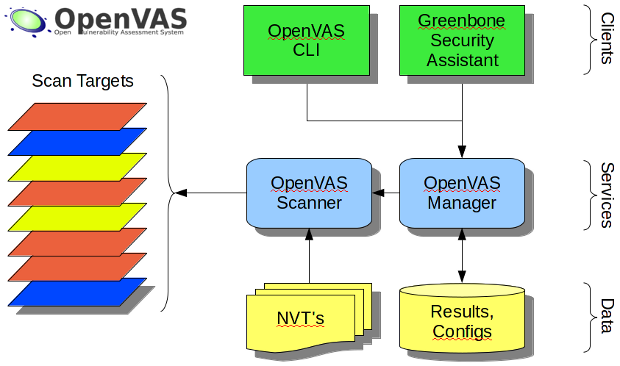
\includegraphics[width=10.0cm]{img/Openvas-structuur.png} \textcite{Openvas-about}
 
De user interface (hierboven vermeld als 'Greenbone Security Assistant') is in veel gevallen een webinterface dat acties doorstuurt naar de manager, zoals een scan starten, of rapporten maken. Het is ook mogelijk om acties door te sturen naar de manager via een command line interface (hierboven vermeld als 'OpenVAS CLI'), dit is handig voor als men scans wil automatiseren.

De manager (hierboven vermeld als 'OpenVAS Manager') staat in voor de communicatie tussen de user interface en de scanner engine. Deze onderhoud ook een database waarin alle configuraties, resultaten, SCAP data, CERT data en NVT's zitten. Het is de job van de manager om deze databank up-to-date te houden zodat deze steeds een volledige vulnerability management oplossing kan bieden.

De scanner (hierboven vermeld als 'OpenVAS Scanner') staat in voor de effectieve scan van een target. Deze heeft een cache waar alle NVT's aanwezig zijn die de scanner nodig heeft om een target te kunnen scannen. Deze geeft zijn resultaten terug aan de manager. 

Indien men een scan start voor een range van machines, zal de scanner engine eerst een 'alive check' uitvoeren op alle hosts in de range. Dit kan bestaan uit een simpele ICMP ping naar de host, tot een range van poorten scannen en kijken of de host reageert op 1 van de requests. 

Indien de host reageert, zal er een port scan gestart worden, de tool die men hiervoor gebruikt is in veel gevallen 'nmap'. De range van poorten wordt op voorhand gedefinieerd door de gebruiker en indien er een firewall aanwezig is, zal hier ook rekening mee gehouden worden. 

De scanner zal hierna een aantal dingen analyseren, zoals het besturingssysteem dat op de host draait, en welke services overeen komen met de open poorten. Als al deze feiten uiteindelijk bekend zijn, zal de scanner op basis van deze analyse NVTs naar de hosts sturen en kijken of deze vatbaar is voor bepaalde exploits \textcite{Qualys}.

Uiteindelijk zal de scanner alle gevonden informatie doorsturen naar de manager, en op basis hiervan een rapport maken die leesbaar is voor de gebruiker.

\subsection{Requirements}

%TODO: wat beter herschrijven
%TODO: functionaliteiten opsommen!

In de volgende delen, zullen we Nessus en Openvas vergelijken op een aantal vlakken dat belangerijk zijn in een scanner. Een aantal belangerijke zaken (snelheid van de scanner, accuraatheid, etc...) zullen pas besproken worden in hoofdstuk~\ref{ch:methodologie}, omdat deze tot mijn onderzoek behoren. Eerst zal er kort een aantal zaken besproken worden zoals de geschiedenis van de scanner, de licenties, de support dat de scanner krijgt en de hardware vereisten. Hierna bespreken we de belangerijkste zaken.

Een volwaardige vulnerabiltiy scanner moet aan een paar voorwarden voldoen, het belangerijkste onderdeel zijn de NVTs. Als deze niet tijdig worden geüpdate, is de scanner niet meer betrouwbaar voor de nieuwste vulnerabilities, en geeft dit een vals veilig gevoel. Hiervoor zullen we 2 grote vulnerabilities (1 voor linux, en 1 voor windows) opzoeken en kijken wanneer beide scanners deze NVT toegevoegd hebben. Voor linux heb ik gekozen voor de 'shellshock' vulnerability (CVE-2014-6271), voor windows is dit 'Server Service Vulnerability' (CVE-2008-4250)

Uiteindelijk bespreken we ook de functionaliteiten van beide scanners. Eerst zullen we bepaalde funtionaliteiten bespreken die een betere performantie geven, of een accurater beeld geven van het systeem. Daarna bespreken we bepaalde functies die niet direct bijdragen tot het eindrapport, maar de scanner gemakkelijker laten implementeren met de bestaande infrastructuur of het grootste deel van het onderhoud automatiseren. 

%TODO: meer testen toevoegen dat impact hebben op eindrapport
Voor het eerste deel gaan we na of beide scanners een 'credential scan' ondersteunen, deze test gebeurt door het inloggen op een bepaalde dienst (meestal ssh) en heeft dus ook de mogelijkheid om configuratie files te controleren op fouten \textcite{Digitalbond}. Een basisvereiste is ook vaak dat scanner meerdere scans tegelijkertijd kunnen uitvoeren, Hoewel dit bij moderne scanners zo goed als steeds het geval is gaan we voor volledigheid dit ook nakijken. Uiteindelijk kijken we ook of de scanner 'agent based' scanning toestaat, dit is een klein programma dat op een host geïnstalleerd word, en commandos van van een centrale machine kan ontvangen. Deze zal een scan uitvoeren op de lokale machine, en zijn resultaten doorsturen naar de centrale machine waar deze beschikbaar is via alle interfaces.

%TOOD: meer testen toevoege ndat GEEn impact hebben op eindrapport 
%TODO: RESP/API uitleggen
Uiteindelijk kijken we of  de server zichzelf onderhoud (zoals NVTs updaten), en wat er nog manueel moet gebeuren. Ook kijken we of er een REST interface, of een API aanwezig is. 
%---------------------------------------------------

\subsection{Nessus}

%TODO: informatie over nessus (prijs,tennable, geschiedenis, edities, support, etc...
%TODO: history citen naar boek V werkt niet voor een reden
%@BOOK{Nessus,
%  TITLE = {Nessus Network Auditing},
%  AUTHOR = {Carey Mark, Russ Roger, Paul Criscuolo, Mike Petruzzi},
%  YEAR = {2008}, 
%  PUBLISHER = {O'reilly},
%}

\subsubsection{Geschiedenis}
Nessus is in 1998 opgericht door Renaud Deraison, met de bedoeling om een gratis vulnerability scanner te maken dat over het internet machines kon scannen. Rond deze software werd het bedrijf tenable opgericht en werd al snel 1 van de populairste oplossingen voor vulnerability managment. Vanaf nessus versie 3 (2005) werd de source code niet meer publiek gemaakt omdat er misbruik van gemaakt werd door de concurrentie. De nessus scanner werd doorverkocht door bedrijven met hun eigen logo en vermelden dat het hun scanner was, ook was er weinig tussenkomst van de community (vooral op gebied van de scanner engine) \textcite{Cnet}.

\subsubsection{Licenties}
Tenable heeft een aantal nessus producten, maar voor deze bachelorproef kijken we naar 'Nessus Professional'. De reden hiervoor is dat dit product zo goed als volledig overeenkomt met een openvas installatie (met een paar limitaties). De licentiekosten hiervoor zijn 2190 \$ / jaar (ongeveer 2010 euro) en is proprietary software.
 
\subsubsection{Support}
Als men een licentie van 'Nessus Professional' heeft, is het mogelijk om support te krijgen via live chat, email en een support portal. Deze zaken zijn 24/7 te benaderen \textcite{Nessus-support}.
 
\subsubsection{Nvt development}
Nessus heeft op moment van schrijven 87.071 plugins \textcite{Nessus-nvt}. Deze NVTS worden geschreven in .nasl (Nessus attack script language).

Voor de shellshock vulnerability is er een NVT verschenen op 24-09-2014 \textcite{Vulners-shellshock-nessus}. Dit is dezelfde dag als shellshock publiek gemaakt werd. De windows vulnerability NVT werd geüpload op 23-10-2008, dit is ook op de dag dat windows de vulnerability publiek maakte.
 

\subsubsection{Functionaliteiten}
\textbf{\textit{Credential scan: }} Deze functionaliteit is beschikbaar, met ondersteuning voor een aantal services. De belangerijste services worden hier opgelijst: database, mongoDB, ssh, windows en SNMPv1/v2c \textcite{Nessus-functions}.

\textbf{\textit{Meerdere scans: }} Dit is mogelijk op elke versie.

\textbf{\textit{Agent based: }} Dit is niet mogelijk met de 'professional' licentie, maar wel met de 'manager' licentie \textcite{Nessus-functions}.
%todo: kijken of nessus cron gebruikt
\textbf{\textit{Onderhoud: }} Op de webinterface is het mogelijk om bepaalde of alle  elementen te updaten. Ook is het mogelijk om een interval in te stellen wanneer deze moet geüpdate worden (dagelijks, wekelijks of maandelijks).

\subsubsection{Hardware}
De minimum systeemvereisten voor een scanner zijn:

\begin{itemize}
\item Dual core 2GHz CPU
\item 2-4 GB RAM
\item 30GB HDD
\end{itemize}

\textcite{Nessus-requirements}

%-------------------------------------------------------------------

\subsection{Openvas}
%%TODO: mailing list uitleggen, IRC?

\subsubsection{Geschiedenis}
Openvas is een fork van de laatste source code die nessus publiek heeft gemaakt (2005), en begon onder de naam \textcite{Securiteam} en werd begonnen door Tim Brown. Dit project is nog steeds volledig opensource \textcite{Openvas-source} en gratis voor zowel personen, als bedrijven met uitzondering op een (niet verplichte) betalende licentie van greenbone voor NVT's \textcite{Openvas-nvt}. De grootste bijdrager voor openvas is greenbone, deze zorgt voor een groot deel van de NVTs, de webinterface en bugfixes \textcite{Openvas-contributors}.

\subsubsection{Licenties}

Openvas valt onder de GPL license, is open-source en is gratis te gebruiken voor zowel personen, als bedrijven.

\subsubsection{Support}
%TODO: monitor IRC chat activity \textcite{Openvas-IRC}.  
Een nadeel van open-source projecten is vaak dat je afhankelijk bent van de community voor support. Dit is bij openvas niet anders, buiten een mailing list is de support zo goed als nietbestaande. De openvas website bevat veel verouderde links zoals een wiki, IRC chat en screenshots. Op het moment van schrijven is de laatste entry in de wiki voor openvas 7 \textcite{Openvas-wiki}, ook op de screenshots pagina is de laatste entry voor openvas 7 \textcite{Openvas-screenshots}.

\subsubsection{Nvt development}
%TODO: worm uitleggen?
Openvas heeft op het moment van schrijven 53.082 plugins \textcite{Openvas-nvt} waarvan er 214 geüpload zijn in de laatste maand. Wat hier ook opvallend is, is dat alle plugins in openvas geschreven worden in nasl (dit staat voor 'nessus attack script language'). Openvas gebruikt dus nog steeds dezelfde code voor NVTs te schrijven als nessus. 

Voor de shellshock vulnerability heeft openvas de NVT geupload op 25-09-2014 \textcite{Vulners-shellshock-openvas}. Dit is 1 dag later als de announcement van shellshock en is gemaakt door greenbone. Dit lijkt onschuldig, maar shellshock heeft 24 uur na de ontdekking al voor het ontstaan van botnets gezorgd \textcite{wired-shellshock}. 

De windows vulnerability werd beschikbaar gesteld op 24-10-2008, Dit is 1 dag na de bekendmaking door windows. Hoewel de gevolgen niet zo erg waren als shellshock, gebruikte de worm \textcite{Microsoft} deze vulnerability om zich te verspreiden.

\subsubsection{Functionaliteiten}
%todo: targets uitleggen?
\textbf{\textit{Credential scan: }} Deze functionaliteit is beschikbaar, maar dit is niet op scan niveau. Dit betekent dat men 2 verschillende targets moet aanmaken als men een credential en een non-credential wil starten (ookal is dit hetzelfde IP). De ondersteunde services zijn hier: SSH, SMB, ESXi en SNMP.

\textbf{\textit{Meerdere scans: }} Dit is mogelijk.

\textbf{\textit{Agent based: }} Dit mogelijk.
%todo: uitleggen wat cron is?
\textbf{\textit{Onderhoud: }} Het is niet mogelijk om in de webinterface updates te starten. De updates (voor alles) worden wel automatisch elke dag geüpdate om 1 uur snachts door middel van cronjobs.

\subsubsection{Hardware}
De minimum systeemvereisten voor openvas staan niet op de site, er is wel een virtuele machine aanwezig voor openvas te testen. De requirements hieronder zijn van deze virtuele machine, in realiteit zullen deze requirements hoger liggen. De reden hiervoor is dat dit een minimale versie is dat bepaalde features niet heeft, ook zijn er nog meer beperkingen zoals dat het besturingssysteem kan niet updaten. Dit is dus niet gepast voor een productie omgeving.

\begin{itemize}
\item Dual core CPU
\item 2 RAM
\item 9GB HDD
\end{itemize}

\textcite{Openvas-requirements}

%-----------------------------------------------------------

\section{Probleemstelling en Onderzoeksvragen}
\label{sec:onderzoeksvragen}

%% TODO:
%% Uit je probleemstelling moet duidelijk zijn dat je onderzoek een meerwaarde
%% heeft voor een concrete doelgroep (bv. een bedrijf).
%%
%% Wees zo concreet mogelijk bij het formuleren van je
%% onderzoeksvra(a)g(en). Een onderzoeksvraag is trouwens iets waar nog
%% niemand op dit moment een antwoord heeft (voor zover je kan nagaan).

\section{Opzet van deze bachelorproef}
\label{sec:opzet-bachelorproef}

%% TODO: Het is gebruikelijk aan het einde van de inleiding een overzicht te
%% geven van de opbouw van de rest van de tekst. Deze sectie bevat al een aanzet
%% die je kan aanvullen/aanpassen in functie van je eigen tekst.

De rest van deze bachelorproef is als volgt opgebouwd:

In Hoofdstuk~\ref{ch:methodologie} wordt de methodologie toegelicht en worden de gebruikte onderzoekstechnieken besproken om een antwoord te kunnen formuleren op de onderzoeksvragen.

%% TODO: Vul hier aan voor je eigen hoofstukken, één of twee zinnen per hoofdstuk

In Hoofdstuk~\ref{ch:conclusie}, tenslotte, wordt de conclusie gegeven en een antwoord geformuleerd op de onderzoeksvragen. Daarbij wordt ook een aanzet gegeven voor toekomstig onderzoek binnen dit domein.


%%=============================================================================
%% Methodologie
%%=============================================================================

\chapter{Methodologie}
\label{ch:methodologie}

%% TODO: Hoe ben je te werk gegaan? Verdeel je onderzoek in grote fasen, en
%% licht in elke fase toe welke stappen je gevolgd hebt. Verantwoord waarom je
%% op deze manier te werk gegaan bent. Je moet kunnen aantonen dat je de best
%% mogelijke manier toegepast hebt om een antwoord te vinden op de
%% onderzoeksvraag.


%section{Studie}

%Voor deze proeven te beginnen, zijn we begonnen met het bestuderen van openvas. De reden hiervoor is dat deze open-source is, en het dus gemakkelijker is om een beeld te krijgen achter de schermen. Nadat de literatuurstudie klaar was, moest er beslist worden hoe het verloop van dit onderzoek zou verlopen. Uitendelijk is er besloten om een gedetailleerd onderzoek te voeren op 

\section{Testen bepalen}

%todo 3de test?
%todo vermelden welke creds gebruikt zijn (ssh voor linux, ? voor windows)
In dit onderzoek zal er met elke scanner 4 scans uitgevoerd worden op elk target. De reden hierachter is dat er in een professionele omgeving 2 punten zijn die belangerijk zijn.Zowel nessus als openvas hebben hiervoor aparte profielen die focussen op een ander deel. Naast deze 2 scans is een credential scan ook een noodzaak om een inzicht te krijgen hoe goed een systeem lokaal beveiligd is (indien men toegang en permissie heeft om deze te scannen met bv. ssh). Voor elke scanner zal er dus een snelle credential, accurate credential, snelle uncredential en een accurate uncredential scan uitgevoerd worden. Dit zal gebeuren in een paar omgevingen die we hieronder bespreken.

Eerst testen we dit op honeypots, dit zijn servers die intentioneel een zwakke configuratie hebben die veel vulnerabilities toont op de scanner. Het doel hiervan is dat deze heel goed opgevolgd moeten worden, en van zodra men activiteit op de server opmerkt dit onderzoeken en kijken of er onbevoegde persoon / malware aanwezig is. Deze test zal bepalen hoeveel vulnerabilities op een zwak systeem gevonden worden voor zowel een linux, als een windows machine.

%SE uitleggen?
Hierna zullen de scanners gebruikt worden om een webserver te scannen over het internet. Deze test is een goede weergave voor een deel van een penetration test. We verwachten op de server zelf weinig tot geen fouten, maar de extra informatie die de scanner ons geeft zoals het besturingssysteem of welke diensten er draaien op het systeem. Deze informatie kan gebruikt worden voor andere aanvallen zoals social engineering.

\section{Opzetten testomgeving}

Voor dit onderzoek werd er gebruik gemaakt van 4 virtuele machines op Virtualbox versie 5.1.10. Voor de virtuele machines waar er een vulnerability scanner op moest draaien, hebben we gebruik gemaakt van een CentOS minimal image. Deze kregen ook dezelfde instellingen die hieronder vermeld worden:

\begin{itemize}
\item 8000 MB ram
\item 4 CPUs
\item NAT \& host-only interfaces
\end{itemize}

Voor de honeypots gebruikten we een iets minder zware virtuele machine, de instellingen hiervoor worden hieronder ook vermeld. 

\begin{itemize}
\item 1000 MB ram
\item 2 CPUs
\item Host-only interface
\end{itemize}

De fysieke computer waar deze testen op zijn uitgevoerd heeft 16GB ram en een cpu met 4 cores en 8 threads. Tijdens de testen waren er geen andere programmas actief die een impact zouden kunnen hebben op de resultaten. Ook werden alleen de machines die getest moeten worden aangezet zodat beide scanners geen impact op elkaar konden hebben.

\section{Installatie}

\subsubsection{Nessus}

%WGET COMMANDO BIJZETTEN, NESSUS VERSIE, NESSUS CLI TESTEN
Voor nessus te downloaden op de virtuele machine (met enkel CLI), moeten we naar de productpagina gaan. Sinds we geen extra software op de virtuele machine wouden (zoals FTP of SMB), zullen we wget gebruiken voor de .rpm file te downloaden. Dit is niet zo simpel, sinds de download link een pop up weergeeft voor de juiste versie te kiezen. Na dit probleem op te zoeken, is het duidelijk dat we bepaalde waarden met wget moeten meegeven \textbf{\textit{COMMAND}}.

Na de installatie van de RPM file (38 MB), poort 8834/tcp te openen in firewall-cmd en de service nessusd te starten is de webinterface bereikbaar. Hier moeten we de licentiecode ingeven die we verkregen hebben bij het aanvragen van een nessus home licentie. Hierna volgt een download scherm dat +- 7 minuten duurt. Hierna kunnen we beginnen met scannen.

\subsubsection{Openvas}

Voor openvas te downloaden op de virtuele machine (met enkel CLI), hebben we 2 opties. We kunnen deze van source compilen, of de \textcite{Openvas-installation}. Wij gebruiken de packages, omdat dit minder tijd in beslag neemt. Voor deze packages te downloaden gebruiken we de atomicorp repository, omdat hiernaar verwezen word op de openvas site.

We installeren de packages voor openvas 9 via yum. De totale grootte van alle packages is 70 MB (185 dependencies). Na deze te downloaden moeten we alles installeren via command line, hiervoor gebruiken we 'openvas-setup'. Deze download eerst alle NVTs (28 MB, verplicht), maar na de download crashed het script omdat we de package 'bzip2' niet geïnstalleerd hebben. We starten het script terug op en merken dat we alle NVTs opnieuw moeten downloaden. Hierna geeft het script een niet fatale error 'certool not found', maar het script gaat verder en blijft vasthangen na 'verify admin password'. Op de achtergrond is het script een databank aan het maken met alle NVTs in, na deze stap is het script gedaan. Het script heeft 23 minuten in beslag genomen.

Na poort 9392/tcp open te zetten in firewall-cmd is het \textit{niet} mogelijk om te connecteren op de webinterface. We gebruiken een ander script 'openvas-check-setup --v9' om te kijken wat er mis is. Deze geeft weer dat de redis server niet gestart is. Deze zit in een failing state, en wil niet herstarten. Na de log files te raadplegen hebben we selinux op 'permissive' gezet, en werkt de redis server nu wel.

Na de check-config nog eens te overlopen, blijkt dat de services van openvas momenteel niet aanstaan. Bij deze opmerkingen staan er tussen haakjes openvassd en openvasmd. Na deze commandos uit te voeren, blijkt de services nog steeds niet te draaien. Na dit verder te onderzoeken, blijkt dat de service openvas-scanner, openvas-manager en gsad noemen. we starten deze op en runnen de check-config opnieuw. 

De config geeft nogmaals een probleem, deze keer omdat de database geen tot weinig gegevens bevat. Hiervoor moeten we het commando 'openvasmd --rebuild' starten. Na 4-5 minuten is deze gedaan en draaien we de check-config nogmaals. Nu geeft deze weer dat er geen SCAP en CERT data aanwezig zijn. Hoewel dit \textit{niet} verplicht is, installeren we deze gegevens voor de volledigheid van de scanner. De sync moet gebeuren met rsync, maar sinds deze sync veel files bevatten die niet groot zijn gaat dit heel traag. Deze duurden samen ongeveer 22 minuten en nemen +-800MB in beslag. 

Als al deze gegevens aanwezig zijn, draaien we het commando check-config nog eens. Deze geeft weer dat selinux moet gedisabled worden. We proberen deze eerst op 'permissive' te zetten, maar het script geeft nog steeds een foutmelding. Na een reboot van de server voor selinux uit te zetten, geeft het script weer dat er een paar packages die \textbf{optioneel} zijn niet aanwezig zijn (zoals alien en net-tools). We installeren deze ook zodat deze geen invloed kunnen hebben op de eindresultaten van de scans.

Uiteindelijk geeft het script weer dat de openvas installatie klaar is voor gebruik. Na het bezoeken van de webinterface blijkt dat dit nog steeds niet mogelijk is. Na te troubleshooten blijkt dat de error in het begin van openvas-setup (certool not found) hier schuldig voor is. Na de package 'gnutls-utils' te installeren en nieuwe certificaten te genereren, is het mogelijk om de webinterface te raadplegen. 

Als we de CLI bekijken, blijkt dat deze niet werkt omdate we niet werken met socket files. We lossen dit op door openvas op localhost te laten luisteren in plaats van een .sock file te gebruiken (openvasmd -a 127.0.0.1), hierna werkt de CLI zoals het hoort.

\subsubsection{Honeypots}

Voor de linux honeypot hebben we 'metasploitable' genomen. Dit is een linux machine die gebaseerd is op ubuntu 8.04 en een reeks services heeft draaien. Deze services zijn opzettelijk zo zwak mogelijk geconfigureerd zodat men op deze virtuele machines vulnerability scanners kunnen testen en zo leren een penetration test uit te voeren.

Voor de windows honeypot hebben we een windows xp machine zonder service packs geïnstalleerd, maar met een aantal servers (SMB,SMTP,SNMP, FTP en IIS). Vooral door deze missende service packs hebben deze veel problemen + er zijn geen opzettelijk slecht geconfigureerde machines zoals metasploitable omdat windows xp onder een licentie valt. 

\subsubsection{Webservers}

Als 2de test zullen we een webserver scannen die momenteel in gebruik is door HoGent. \textit{\textbf{*URLS*}}. Hiervoor hebben we een schriftelijke toestemming gekregen door Van Vreckem Bert.

\section{Instellingen scans}

\section{Scan resultaten}

\section{Scan resultaten valideren}

 %db(underscore)autopwn methode gebruiken (in metasploit) om false positives niet manueel te moeten filteren?

\section{Analyseren van de data}

%alle gevonden data in een tabel gieten, voor en nadelen nog is opsommen en \textit{persoonlijke mening geven?}

%% Voeg hier je eigen hoofdstukken toe die de ``corpus'' van je bachelorproef
%% vormen. De structuur en titels hangen af van je eigen onderzoek. Je kan bv.
%% elke fase in je onderzoek in een apart hoofdstuk bespreken.

%\input{}
%\input{}
%...

%%=============================================================================
%% Conclusie
%%=============================================================================

\chapter{Conclusie}
\label{ch:conclusie}

%% TODO: Trek een duidelijke conclusie, in de vorm van een antwoord op de
%% onderzoeksvra(a)g(en). Wat was jouw bijdrage aan het onderzoeksdomein en
%% hoe biedt dit meerwaarde aan het vakgebied/doelgroep? Reflecteer kritisch
%% over het resultaat. Had je deze uitkomst verwacht? Zijn er zaken die nog
%% niet duidelijk zijn? Heeft het ondezoek geleid tot nieuwe vragen die
%% uitnodigen tot verder onderzoek?


%%---------- Back matter ------------------------------------------------------

\printbibliography
\addcontentsline{toc}{chapter}{\textcolor{maincolor}{\IfLanguageName{dutch}{Bibliografie}{Bibliography}}}


\listoffigures
\listoftables

\end{document}
